\documentclass[UTF8]{ctexart}
\usepackage{geometry}
\usepackage{amsmath}
\usepackage{graphicx} %插入图片的宏包
\usepackage{float} %设置图片浮动位置的宏包
\geometry{a4paper,scale=0.8}
\sectionfont{\bfseries\Large\raggedright}

\title{machine learning笔记}
\author{徐世桐}
\date{}
\begin{document}
\maketitle

% ----------------------------------------------------------------------
% |                              基础定义                               |
% ----------------------------------------------------------------------
\section{基础定义}
\noindent \textbf{二元分类}:输出分类个数为2\\
\textbf{多元分类}:输出分类个数不限

  $one-versus-the-rest$ OvR:计算属于每一分类的可能性,取可能性最大的分类为输出分类

  $one-versus-one$ OvO:对所有分类两两使用二元分类,每一分类器训练只需一部分数据\\
\textbf{multilabel多标签分类}:目标检测,对一图像中的物体加label\\
\textbf{multioutput多类分类}:多标签分类,每一标签可包含多种信息\\
\textbf{MSE} = $\frac{1}{m}\sum_{i=1}^{m}(x^{(i)} - y^{(i)})^2$\\
\textbf{learning schedule}:根据迭代次数更新学习率\\
\textbf{rigid regression}:回归方法,$J(\theta) = MSE(\theta) + \frac{\alpha}{2}\sum_{i}\theta_i^2$

  降低所有权重值\\
\textbf{lasso regression}:回归方法,$J(\theta) = MSE(\theta) + \alpha \sum_i |\theta_i|$

  降低不重要的权重值\\
\textbf{elastic net}:回归方法,$J(\theta) = MSE(\theta) + \gamma\alpha \sum_i |\theta_i| + (1-\gamma)\frac{\alpha}{2}\sum_{i}\theta_i^2$\\
\textbf{early stopping}:提早结束训练

  对于每一epoch,当验证集MSE值增高时,证明开始overfit,停止训练

  即在epoch-error图中泛化误差最低时停止训练\\
\textbf{在训练中使用正则化代价函数,训练结束后测试中代价函数不使用正则化项}

% ----------------------------------------------------------------------
% |                              数学计算                               |
% ----------------------------------------------------------------------
\section{数学计算}
\noindent \textbf{pseudo inverse}:

  对矩阵$X=USV^T$,pseudo inverse $X^+=VS^+U^T$。$S^+$求法:

  \quad 1.对所有$S$元素,接近0的值赋为0

  \quad 2.对所有非零元素取倒数

  \quad 3.取矩阵转置,得到$S^+$

% ----------------------------------------------------------------------
% |                              分析结果                                |
% ----------------------------------------------------------------------
\section{分析结果}
\noindent \textbf{confusion matrix困惑矩阵}:分析二元/多元分类
  
  $\begin{bmatrix}
    TN & FP \\
    FN & TP
  \end{bmatrix}$

  一行对应同一期望输出,一列对应同一计算输出

  $T/F$: 此位置的计算输出是否和预计输出一致

  $P/N$: 此位置的预计输出是否为真

  \textbf{precision} $= \frac{TP}{TP + FP}$

  \quad 即$P($计算结果匹配 $|$ 计算结果为正$)$

  \textbf{recall} = $\frac{TP}{TP + FN}$

  \quad 即$P($计算结果匹配 $|$ 预计结果为正$)$

  \textbf{$F_1$} $= \frac{2}{\frac{1}{precision} + \frac{1}{recall}}$ 
  
  \quad precision 和 recall的调和平均值
  
  \textbf{specificity} = $\frac{TN}{TN + FN}$\\
\textbf{ROC curve}:分析二元/多元分类

  \begin{figure}[H] %H为当前位置,!htb为忽略美学标准,htbp为浮动图形
    \centering %图片居中
    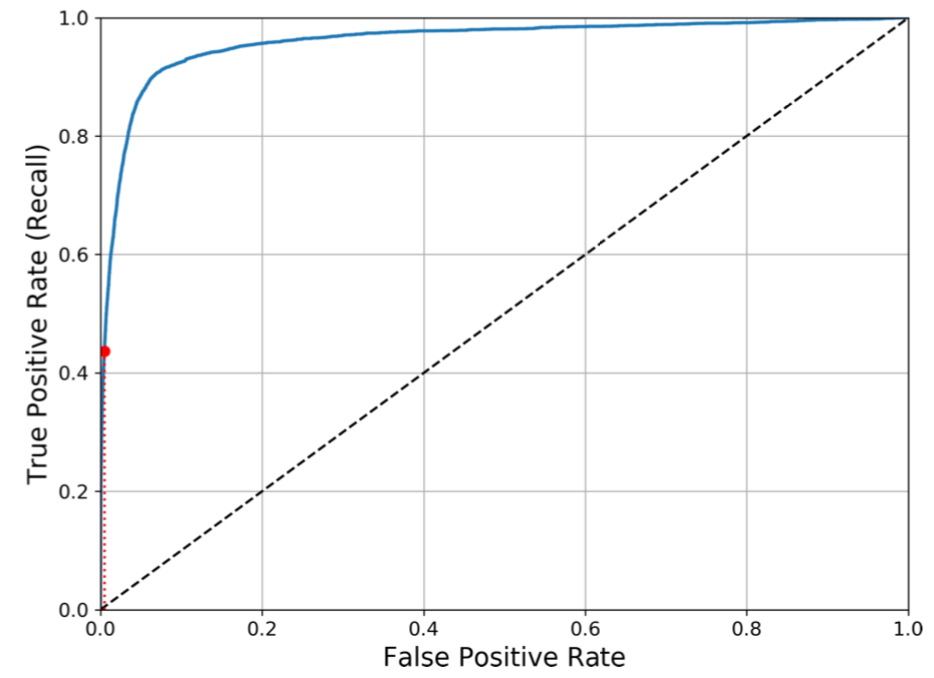
\includegraphics[width=0.3\textwidth]{note_images/ROC_curve.png} %插入图片,[]中设置图片大小,{}中是图片文件名
  \end{figure}

  y轴recall值,x轴false positive rate$FPR = \frac{FN}{FN + TN} = \frac{FN}{1-specificity}$

  期望的ROC curve为recall从0快速增长到1。并保持直到$FPR$为1。
  
  \quad 即期望曲线下方面积接近1\\
\textbf{learning curves}:观察模型是否有over underfit

  \begin{figure}[H] %H为当前位置,!htb为忽略美学标准,htbp为浮动图形
    \centering %图片居中
    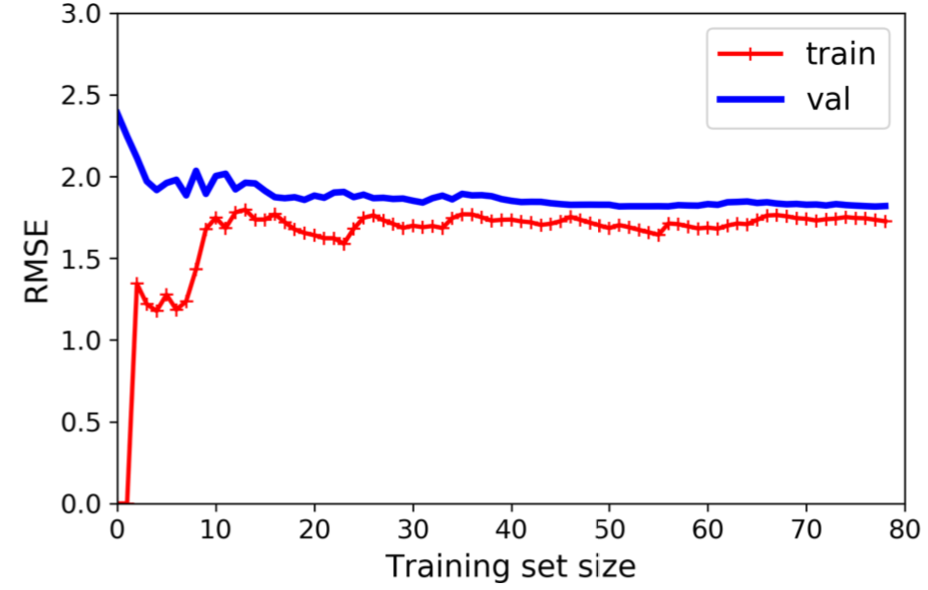
\includegraphics[width=0.3\textwidth]{note_images/learning_curve.png} %插入图片,[]中设置图片大小,{}中是图片文件名
  \end{figure}

  x轴为\textbf{一整次训练(包含多次epoch)使用的训练集大小},y轴为root MSE。

  画出训练集\ 测试集在使用不同训练集大小后的root MSE。

  分析:

  \quad 期望2曲线平缓值低且相近,

  \quad 当2曲线平缓值差值较大,测试集平缓值较低,则过拟合

  \quad 当2曲线平缓值较高,则欠拟合\\
\textbf{模型复杂度-error epoch-error}:

  \begin{figure}[H] %H为当前位置,!htb为忽略美学标准,htbp为浮动图形
    \centering %图片居中
    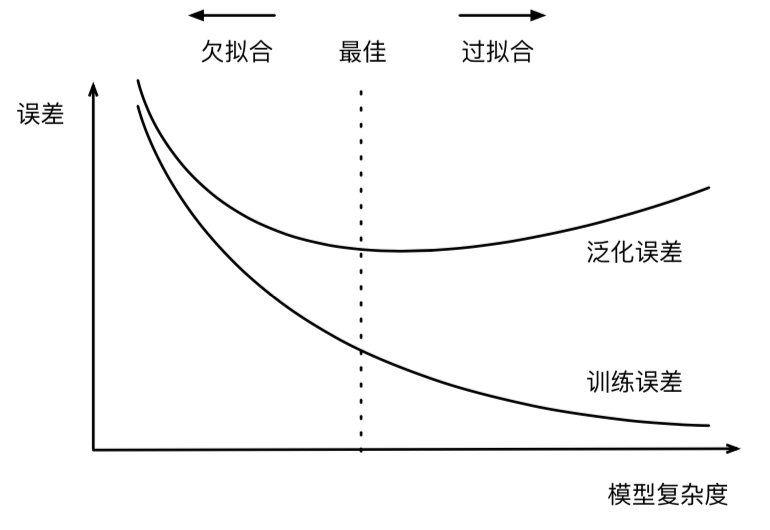
\includegraphics[width=0.3\textwidth]{note_images/epoch-complex-error.png} %插入图片,[]中设置图片大小,{}中是图片文件名
  \end{figure}

  2种图,形状类似,x轴内容不同
\end{document}
